% Options for packages loaded elsewhere
\PassOptionsToPackage{unicode}{hyperref}
\PassOptionsToPackage{hyphens}{url}
%
\documentclass[
]{article}
\usepackage{amsmath,amssymb}
\usepackage{iftex}
\ifPDFTeX
  \usepackage[T1]{fontenc}
  \usepackage[utf8]{inputenc}
  \usepackage{textcomp} % provide euro and other symbols
\else % if luatex or xetex
  \usepackage{unicode-math} % this also loads fontspec
  \defaultfontfeatures{Scale=MatchLowercase}
  \defaultfontfeatures[\rmfamily]{Ligatures=TeX,Scale=1}
\fi
\usepackage{lmodern}
\ifPDFTeX\else
  % xetex/luatex font selection
\fi
% Use upquote if available, for straight quotes in verbatim environments
\IfFileExists{upquote.sty}{\usepackage{upquote}}{}
\IfFileExists{microtype.sty}{% use microtype if available
  \usepackage[]{microtype}
  \UseMicrotypeSet[protrusion]{basicmath} % disable protrusion for tt fonts
}{}
\makeatletter
\@ifundefined{KOMAClassName}{% if non-KOMA class
  \IfFileExists{parskip.sty}{%
    \usepackage{parskip}
  }{% else
    \setlength{\parindent}{0pt}
    \setlength{\parskip}{6pt plus 2pt minus 1pt}}
}{% if KOMA class
  \KOMAoptions{parskip=half}}
\makeatother
\usepackage{xcolor}
\usepackage[margin=1in]{geometry}
\usepackage{color}
\usepackage{fancyvrb}
\newcommand{\VerbBar}{|}
\newcommand{\VERB}{\Verb[commandchars=\\\{\}]}
\DefineVerbatimEnvironment{Highlighting}{Verbatim}{commandchars=\\\{\}}
% Add ',fontsize=\small' for more characters per line
\usepackage{framed}
\definecolor{shadecolor}{RGB}{248,248,248}
\newenvironment{Shaded}{\begin{snugshade}}{\end{snugshade}}
\newcommand{\AlertTok}[1]{\textcolor[rgb]{0.94,0.16,0.16}{#1}}
\newcommand{\AnnotationTok}[1]{\textcolor[rgb]{0.56,0.35,0.01}{\textbf{\textit{#1}}}}
\newcommand{\AttributeTok}[1]{\textcolor[rgb]{0.13,0.29,0.53}{#1}}
\newcommand{\BaseNTok}[1]{\textcolor[rgb]{0.00,0.00,0.81}{#1}}
\newcommand{\BuiltInTok}[1]{#1}
\newcommand{\CharTok}[1]{\textcolor[rgb]{0.31,0.60,0.02}{#1}}
\newcommand{\CommentTok}[1]{\textcolor[rgb]{0.56,0.35,0.01}{\textit{#1}}}
\newcommand{\CommentVarTok}[1]{\textcolor[rgb]{0.56,0.35,0.01}{\textbf{\textit{#1}}}}
\newcommand{\ConstantTok}[1]{\textcolor[rgb]{0.56,0.35,0.01}{#1}}
\newcommand{\ControlFlowTok}[1]{\textcolor[rgb]{0.13,0.29,0.53}{\textbf{#1}}}
\newcommand{\DataTypeTok}[1]{\textcolor[rgb]{0.13,0.29,0.53}{#1}}
\newcommand{\DecValTok}[1]{\textcolor[rgb]{0.00,0.00,0.81}{#1}}
\newcommand{\DocumentationTok}[1]{\textcolor[rgb]{0.56,0.35,0.01}{\textbf{\textit{#1}}}}
\newcommand{\ErrorTok}[1]{\textcolor[rgb]{0.64,0.00,0.00}{\textbf{#1}}}
\newcommand{\ExtensionTok}[1]{#1}
\newcommand{\FloatTok}[1]{\textcolor[rgb]{0.00,0.00,0.81}{#1}}
\newcommand{\FunctionTok}[1]{\textcolor[rgb]{0.13,0.29,0.53}{\textbf{#1}}}
\newcommand{\ImportTok}[1]{#1}
\newcommand{\InformationTok}[1]{\textcolor[rgb]{0.56,0.35,0.01}{\textbf{\textit{#1}}}}
\newcommand{\KeywordTok}[1]{\textcolor[rgb]{0.13,0.29,0.53}{\textbf{#1}}}
\newcommand{\NormalTok}[1]{#1}
\newcommand{\OperatorTok}[1]{\textcolor[rgb]{0.81,0.36,0.00}{\textbf{#1}}}
\newcommand{\OtherTok}[1]{\textcolor[rgb]{0.56,0.35,0.01}{#1}}
\newcommand{\PreprocessorTok}[1]{\textcolor[rgb]{0.56,0.35,0.01}{\textit{#1}}}
\newcommand{\RegionMarkerTok}[1]{#1}
\newcommand{\SpecialCharTok}[1]{\textcolor[rgb]{0.81,0.36,0.00}{\textbf{#1}}}
\newcommand{\SpecialStringTok}[1]{\textcolor[rgb]{0.31,0.60,0.02}{#1}}
\newcommand{\StringTok}[1]{\textcolor[rgb]{0.31,0.60,0.02}{#1}}
\newcommand{\VariableTok}[1]{\textcolor[rgb]{0.00,0.00,0.00}{#1}}
\newcommand{\VerbatimStringTok}[1]{\textcolor[rgb]{0.31,0.60,0.02}{#1}}
\newcommand{\WarningTok}[1]{\textcolor[rgb]{0.56,0.35,0.01}{\textbf{\textit{#1}}}}
\usepackage{longtable,booktabs,array}
\usepackage{calc} % for calculating minipage widths
% Correct order of tables after \paragraph or \subparagraph
\usepackage{etoolbox}
\makeatletter
\patchcmd\longtable{\par}{\if@noskipsec\mbox{}\fi\par}{}{}
\makeatother
% Allow footnotes in longtable head/foot
\IfFileExists{footnotehyper.sty}{\usepackage{footnotehyper}}{\usepackage{footnote}}
\makesavenoteenv{longtable}
\usepackage{graphicx}
\makeatletter
\def\maxwidth{\ifdim\Gin@nat@width>\linewidth\linewidth\else\Gin@nat@width\fi}
\def\maxheight{\ifdim\Gin@nat@height>\textheight\textheight\else\Gin@nat@height\fi}
\makeatother
% Scale images if necessary, so that they will not overflow the page
% margins by default, and it is still possible to overwrite the defaults
% using explicit options in \includegraphics[width, height, ...]{}
\setkeys{Gin}{width=\maxwidth,height=\maxheight,keepaspectratio}
% Set default figure placement to htbp
\makeatletter
\def\fps@figure{htbp}
\makeatother
\setlength{\emergencystretch}{3em} % prevent overfull lines
\providecommand{\tightlist}{%
  \setlength{\itemsep}{0pt}\setlength{\parskip}{0pt}}
\setcounter{secnumdepth}{-\maxdimen} % remove section numbering
\ifLuaTeX
  \usepackage{selnolig}  % disable illegal ligatures
\fi
\usepackage{bookmark}
\IfFileExists{xurl.sty}{\usepackage{xurl}}{} % add URL line breaks if available
\urlstyle{same}
\hypersetup{
  pdfauthor={MAUCO},
  hidelinks,
  pdfcreator={LaTeX via pandoc}}

\author{MAUCO}
\date{2024-04-09}

\begin{document}

{
\setcounter{tocdepth}{2}
\tableofcontents
}
\section{\texorpdfstring{\textbf{Manual básico de
R}}{Manual básico de R}}\label{manual-buxe1sico-de-r}

Este manual tiene como finalidad ser una guía básica del uso del
ambiente Rstudio cloud para los investigadores y/o colaboradores que han
solicitado datos pertenecientes a la \emph{Cohorte MAUCO}.

\section{\texorpdfstring{\textbf{Inicio de Sesión en la
plataforma}}{Inicio de Sesión en la plataforma}}\label{inicio-de-sesiuxf3n-en-la-plataforma}

Para iniciar sesión en RStudio Cloud, sigue estos pasos:

\begin{enumerate}
\def\labelenumi{\arabic{enumi}.}
\item
  Abre tu navegador web y ve a la página de inicio de
  \href{https://rstudio.mauco.org/}{RStudio Cloud MAUCO}.
\item
  Una vez en la página de inicio, ingresa tu nombre de usuario en el
  campo \textbf{Username} y tu contraseña en el campo \textbf{Password}.
\item
  Después de ingresar tu información de inicio de sesión, haz clic en el
  botón \textbf{Sign In} para acceder a tu cuenta.
\item
  Si la información de inicio de sesión son correctos, se te dirigirá a
  tu espacio de trabajo en RStudio Cloud, donde podrás acceder a tus
  proyectos y comenzar a trabajar con los datos solicitados.
\end{enumerate}

\section{\texorpdfstring{\textbf{Entorno RStudio
Cloud}}{Entorno RStudio Cloud}}\label{entorno-rstudio-cloud}

El entorno de trabajo de RStudio Cloud se subdivide en una serie de
secciones o regiones, las cuales se enlistan a continuación y pueden
visualizarse en la \textbf{Figura 3.1}.

\textbf{1. La barra de tareas}\\
\textbf{2. El editor de scripts (source)}\\
\textbf{3. Paneles de ambiente e historial}\\
\textbf{4. La consola}\\
\textbf{5. Paneles de archivos (files) y gráficos (plots)}

\begin{figure}

{\centering 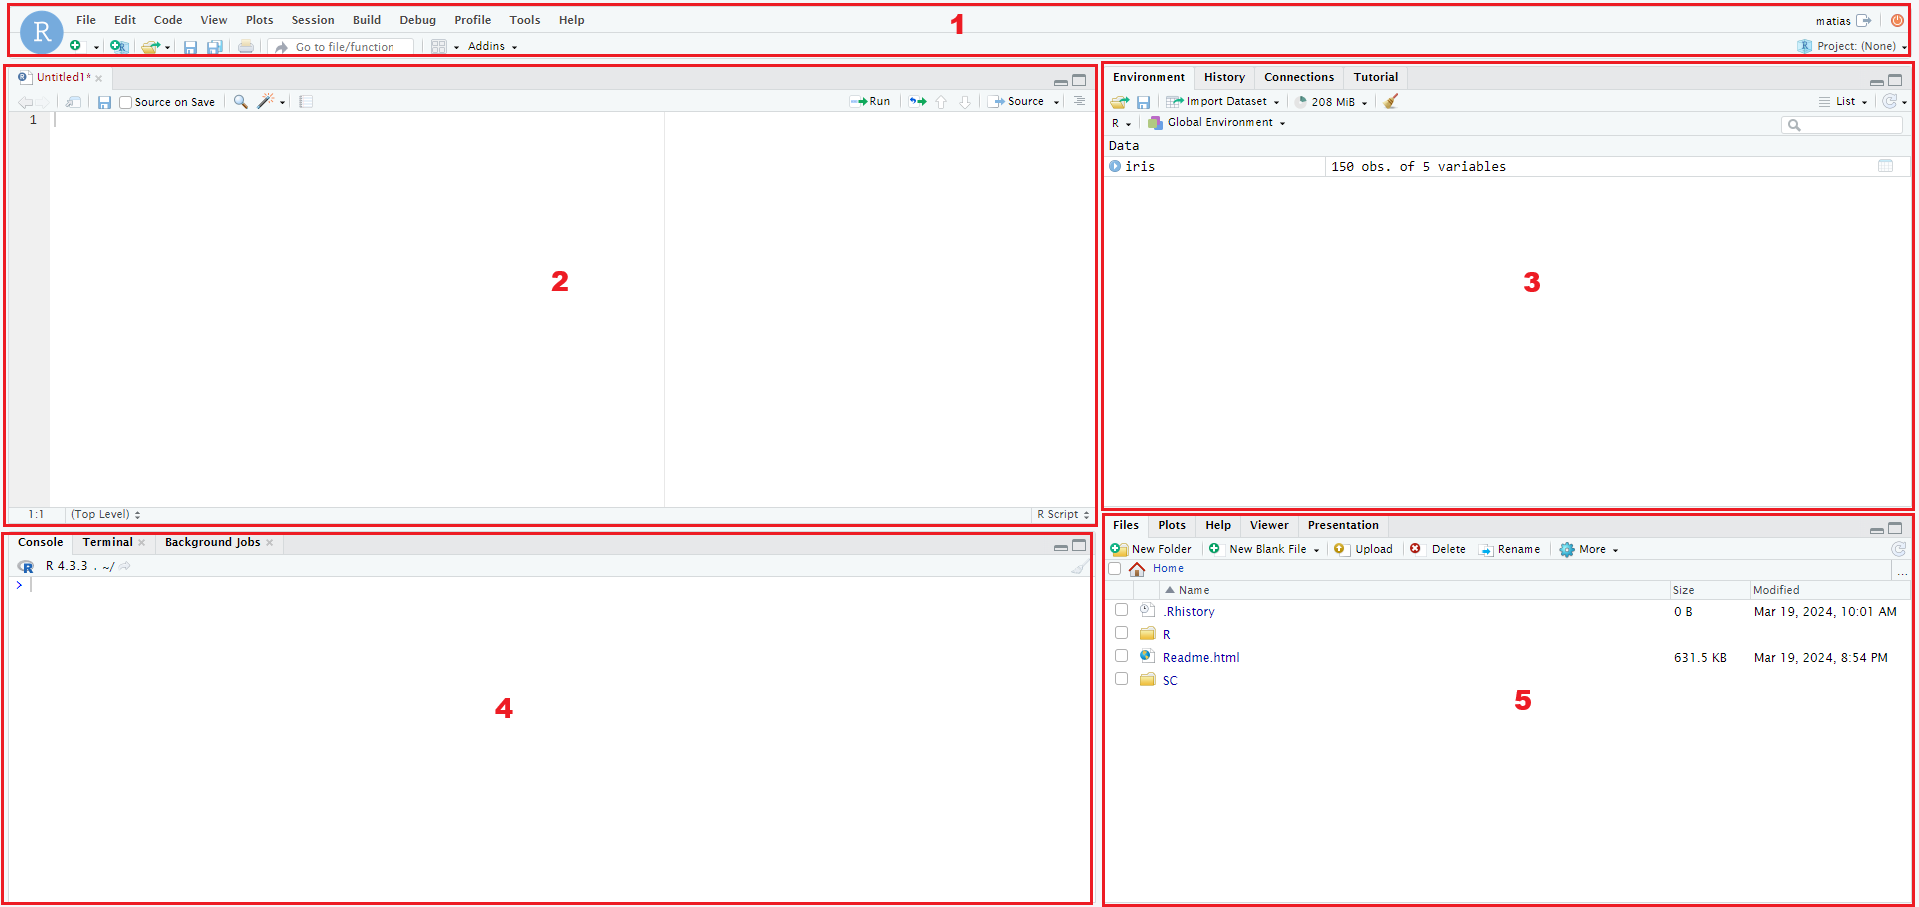
\includegraphics[width=2000px]{images/entorno_num} 

}

\caption{Figura 3.1: Entorno de trabajo RStudio Cloud.  
1. Barra de tareas, 2. Editor de Scripts, 3. Paneles de ambiente e historial, 4. Consola, 5. Paneles de archivos y gráficos.}\label{fig:entorno}
\end{figure}

\subsection{Barra de tareas}\label{barra-de-tareas}

La barra de herramientas de RStudio se encuentra en la parte superior de
la interfaz y proporciona acceso rápido a diversas funciones y
herramientas útiles para trabajar con R y proyectos de análisis de
datos. A continuación, se presenta una descripción de las principales
opciones que puedes encontrar en la barra de tareas:

\begin{itemize}
\item
  File (Archivo): Esta opción te permite realizar operaciones
  relacionadas con archivos, como crear, abrir y guardar scripts de R,
  así como abrir proyectos existentes y cerrar sesiones.
\item
  Edit (Edición): Aquí encontrarás opciones para realizar acciones de
  edición de texto en el editor de scripts, como copiar, pegar,
  deshacer, rehacer y buscar texto.
\item
  Code (Código): Esta opción proporciona herramientas para trabajar con
  código, como ejecutar selecciones de código, comentar o descomentar
  bloques de código, y ajustar el formato del código.
\item
  View (Ver): Te permite cambiar entre diferentes vistas dentro de
  RStudio, como alternar entre la vista de consola y la vista de
  scripts, así como mostrar u ocultar diferentes paneles y ventanas.
\item
  Build (Construir): Aquí encontrarás herramientas relacionadas con la
  construcción de proyectos, como la opción para compilar y cargar
  paquetes, así como la generación de documentos y la creación de
  presentaciones.
\item
  Debug (Depurar): Esta opción proporciona herramientas para depurar y
  rastrear errores en tu código, como establecer puntos de interrupción,
  ejecutar el código paso a paso y verificar el entorno de ejecución.
\item
  Profile (Perfil): Esta opción te permite acceder y gestionar tu perfil
  de usuario.
\item
  Tools (Herramientas): Aquí encontrarás acceso a diversas herramientas
  adicionales, como el instalador de paquetes, el administrador de
  conexiones de base de datos, y la terminal de comandos.
\item
  Help (Ayuda): Te proporciona acceso rápido a la documentación y ayuda
  relacionada con R y RStudio, incluyendo enlaces a la documentación
  oficial, foros de ayuda y recursos adicionales.
\end{itemize}

\subsection{Editor de scripts}\label{editor-de-scripts}

El editor de scripts (Source) en RStudio Cloud es una herramienta
central para escribir, editar y ejecutar código en R.

Con el editor de scripts, podras crear y modificar archivos de script
(.R) de manera eficiente, permitiendo una programación estructurada y
organizada. Además, el editor facilita la ejecución de código, ya sea
línea por línea o en su totalidad, lo que te permitirá probar y depurar
su código de manera interactiva.

En resumen, el editor de scripts en RStudio Cloud es una herramienta que
facilita el desarrollo y la ejecución de código en R, proporcionando un
entorno intuitivo y funcional para trabajar en proyectos de análisis de
datos y estadísticas.

\subsection{Ambiente e historial}\label{ambiente-e-historial}

El Ambiente (Environment) y el Historial (History) son dos paneles
importantes que ofrecen información y funcionalidades clave para el
desarrollo de proyectos en R.

El panel Ambiente (Environment) muestra información sobre las
\textbf{variables} y \textbf{funciones} que están actualmente cargadas
en la sesión de R. Proporciona una visión general de los objetos
existentes en el \textbf{entorno de trabajo} (Workspace), incluyendo sus
\emph{nombres}, \emph{tipos de datos} y \emph{valores actuales}. Este
panel es útil para monitorear y gestionar variables durante el
desarrollo de un proyecto, lo cual permite inspeccionar y manipular
datos en tiempo real.

El panel Historial (History) registra los comandos que han sido
ejecutados en la sesión actual de R. Muestra una lista cronológica de
los comandos previamente ingresados por el usuario, junto con los
resultados correspondientes si los hubiera. Esto facilita la revisión y
reproducción de acciones previas, lo que puede ser útil para recordar
pasos específicos.

\subsection{Consola}\label{consola}

La consola en RStudio Cloud es el espacio interactivo donde puedes
escribir y ejecutar comandos de R en tiempo real. Es el lugar donde se
muestra la salida de los comandos y los mensajes de error, lo que
permite a los usuarios interactuar directamente con el lenguaje de
programación R.

\subsection{Archivos y gráficos}\label{archivos-y-gruxe1ficos}

El panel de archivos (files) proporciona una interfaz visual para
explorar y gestionar los archivos y directorios en tu proyecto. Te
permite navegar por la estructura de archivos, crear nuevos archivos,
importar scripts y organizar tu trabajo de manera eficiente. Además,
este panel facilita la búsqueda y manipulación de archivos, lo que ayuda
a los usuarios a mantener sus proyectos organizados y bien
estructurados.

Por otro lado, el panel de gráficos (plots) muestra los gráficos y
visualizaciones generados durante tu sesión de R. Es un espacio dedicado
para explorar y examinar tus resultados visuales de manera interactiva.
Desde este panel, puedes visualizar gráficos y exportar imágenes.

\section{\texorpdfstring{\textbf{Carga de base de datos en el espacio de
trabajo}}{Carga de base de datos en el espacio de trabajo}}\label{carga-de-base-de-datos-en-el-espacio-de-trabajo}

Luego de haber iniciado a tu sesión de RStudio CLoud, deberas
identificar en el panel de archivos (files) la base datos con la cual
realizarás tus futuros análisis. Las bases de datos pueden encontrarse
en un sin fin de extensiones de archivos.

A continuación se explicara como cargar la base de datos en el espacio
de trabajo (panel environment) para las extensiones de archivos más
utilizadas.

\subsection{\texorpdfstring{Base de datos en archivo con extensión
\emph{.RData}}{Base de datos en archivo con extensión .RData}}\label{base-de-datos-en-archivo-con-extensiuxf3n-.rdata}

La extensión \texttt{.RData} es una extensión de archivos propia del
lenguaje R. Este archivo permite almacenar distintos objetos de R en un
solo archivo. En terminos generales, todos los elementos que maneja R
son objetos, dentro de los cuales pueden ser:

\begin{itemize}
\tightlist
\item
  Valores numéricos
\item
  Vectores
\item
  Matrices
\item
  Funciones
\item
  Bases de datos
\item
  Gráficos
\item
  Entre otros\ldots{}
\end{itemize}

Si en su panel de archivos tiene un archivo con extensión
\texttt{.RData}, puede cargar todos los objetos almacenados en dicho
archivo utilizando el siguiente comando

\begin{Shaded}
\begin{Highlighting}[]
\FunctionTok{load}\NormalTok{(}\StringTok{"nombre\_archivo.Rdata"}\NormalTok{)}
\end{Highlighting}
\end{Shaded}

Así, todos los objetos almacenados en su archivo \texttt{.RData}seran
cargados en su espacio de trabajo.

\subsection{\texorpdfstring{Base de datos en archivo con extensión
\emph{.csv}}{Base de datos en archivo con extensión .csv}}\label{base-de-datos-en-archivo-con-extensiuxf3n-.csv}

Si dispone de un archivo con extensión \texttt{.csv} en su panel de
archivos, podra cargarlo en su espacio de trabajo con la función
\texttt{read.csv()}.

En el siguiente ejemplo, se presenta un caso de uso con la base de datos
\texttt{penguins.csv}.

\begin{Shaded}
\begin{Highlighting}[]
\NormalTok{db\_penguins }\OtherTok{\textless{}{-}} \FunctionTok{read.csv}\NormalTok{(}\AttributeTok{file =} \StringTok{"data/penguins.csv"}\NormalTok{,}
                        \AttributeTok{header =}\NormalTok{ T,}
                        \AttributeTok{sep =} \StringTok{","}\NormalTok{)}
\end{Highlighting}
\end{Shaded}

\begin{longtable}[]{@{}
  >{\centering\arraybackslash}p{(\columnwidth - 16\tabcolsep) * \real{0.0673}}
  >{\centering\arraybackslash}p{(\columnwidth - 16\tabcolsep) * \real{0.0865}}
  >{\centering\arraybackslash}p{(\columnwidth - 16\tabcolsep) * \real{0.1058}}
  >{\centering\arraybackslash}p{(\columnwidth - 16\tabcolsep) * \real{0.1538}}
  >{\centering\arraybackslash}p{(\columnwidth - 16\tabcolsep) * \real{0.1442}}
  >{\centering\arraybackslash}p{(\columnwidth - 16\tabcolsep) * \real{0.1827}}
  >{\centering\arraybackslash}p{(\columnwidth - 16\tabcolsep) * \real{0.1250}}
  >{\centering\arraybackslash}p{(\columnwidth - 16\tabcolsep) * \real{0.0769}}
  >{\centering\arraybackslash}p{(\columnwidth - 16\tabcolsep) * \real{0.0577}}@{}}
\caption{Base de datos penguins desde archivo .csv}\tabularnewline
\toprule\noalign{}
\begin{minipage}[b]{\linewidth}\centering
rowid
\end{minipage} & \begin{minipage}[b]{\linewidth}\centering
species
\end{minipage} & \begin{minipage}[b]{\linewidth}\centering
island
\end{minipage} & \begin{minipage}[b]{\linewidth}\centering
bill\_length\_mm
\end{minipage} & \begin{minipage}[b]{\linewidth}\centering
bill\_depth\_mm
\end{minipage} & \begin{minipage}[b]{\linewidth}\centering
flipper\_length\_mm
\end{minipage} & \begin{minipage}[b]{\linewidth}\centering
body\_mass\_g
\end{minipage} & \begin{minipage}[b]{\linewidth}\centering
sex
\end{minipage} & \begin{minipage}[b]{\linewidth}\centering
year
\end{minipage} \\
\midrule\noalign{}
\endfirsthead
\toprule\noalign{}
\begin{minipage}[b]{\linewidth}\centering
rowid
\end{minipage} & \begin{minipage}[b]{\linewidth}\centering
species
\end{minipage} & \begin{minipage}[b]{\linewidth}\centering
island
\end{minipage} & \begin{minipage}[b]{\linewidth}\centering
bill\_length\_mm
\end{minipage} & \begin{minipage}[b]{\linewidth}\centering
bill\_depth\_mm
\end{minipage} & \begin{minipage}[b]{\linewidth}\centering
flipper\_length\_mm
\end{minipage} & \begin{minipage}[b]{\linewidth}\centering
body\_mass\_g
\end{minipage} & \begin{minipage}[b]{\linewidth}\centering
sex
\end{minipage} & \begin{minipage}[b]{\linewidth}\centering
year
\end{minipage} \\
\midrule\noalign{}
\endhead
\bottomrule\noalign{}
\endlastfoot
1 & Adelie & Torgersen & 39.1 & 18.7 & 181 & 3750 & male & 2007 \\
2 & Adelie & Torgersen & 39.5 & 17.4 & 186 & 3800 & female & 2007 \\
3 & Adelie & Torgersen & 40.3 & 18.0 & 195 & 3250 & female & 2007 \\
4 & Adelie & Torgersen & NA & NA & NA & NA & NA & 2007 \\
5 & Adelie & Torgersen & 36.7 & 19.3 & 193 & 3450 & female & 2007 \\
6 & Adelie & Torgersen & 39.3 & 20.6 & 190 & 3650 & male & 2007 \\
\end{longtable}

La base de datos se almacena en el objeto \texttt{db\_penguins}. Además,
se utilizan tres argumentos de la función \texttt{read.csv()}. El
argumento \texttt{file} permite indicarle a la función la ruta del
archivo dentro de nuestro directorio de trabajo. El argumento
\texttt{header} permite indicarle a la función que nuestra base de datos
disponde de encabezados de columna, utilizando un valor booleano T
(True). Finalmente, el argumento \texttt{sep} permite indicar el signo
empleado para la separación de valores dentro del archivo csv.

\subsection{\texorpdfstring{Base de datos en archivo con extensión
\emph{.xlsx}}{Base de datos en archivo con extensión .xlsx}}\label{base-de-datos-en-archivo-con-extensiuxf3n-.xlsx}

Para cargar una base de datos con la extensión \texttt{.xlsx}, se
recomienda el uso de la función \texttt{read\_xlsx()} de la libreria
\texttt{readxl}.

Primero, cargue la libreria a su entorno de trabajo. Luego, utilize la
función \texttt{read\_xlsx()} como se muestra en el siguiente ejemplo
con la base de datos penguins.

\begin{Shaded}
\begin{Highlighting}[]
\FunctionTok{library}\NormalTok{(readxl)}

\NormalTok{db\_penguins }\OtherTok{\textless{}{-}} \FunctionTok{read\_xlsx}\NormalTok{(}\AttributeTok{path =} \StringTok{"data/penguins.xlsx"}\NormalTok{,}
                         \AttributeTok{sheet =} \StringTok{"Hoja1"}\NormalTok{)}
\end{Highlighting}
\end{Shaded}

\begin{longtable}[]{@{}
  >{\raggedleft\arraybackslash}p{(\columnwidth - 16\tabcolsep) * \real{0.0632}}
  >{\raggedright\arraybackslash}p{(\columnwidth - 16\tabcolsep) * \real{0.0842}}
  >{\raggedright\arraybackslash}p{(\columnwidth - 16\tabcolsep) * \real{0.1053}}
  >{\raggedleft\arraybackslash}p{(\columnwidth - 16\tabcolsep) * \real{0.1579}}
  >{\raggedleft\arraybackslash}p{(\columnwidth - 16\tabcolsep) * \real{0.1474}}
  >{\raggedleft\arraybackslash}p{(\columnwidth - 16\tabcolsep) * \real{0.1895}}
  >{\raggedleft\arraybackslash}p{(\columnwidth - 16\tabcolsep) * \real{0.1263}}
  >{\raggedright\arraybackslash}p{(\columnwidth - 16\tabcolsep) * \real{0.0737}}
  >{\raggedleft\arraybackslash}p{(\columnwidth - 16\tabcolsep) * \real{0.0526}}@{}}
\caption{Base de datos penguins desde archivo .xlsx}\tabularnewline
\toprule\noalign{}
\begin{minipage}[b]{\linewidth}\raggedleft
rowid
\end{minipage} & \begin{minipage}[b]{\linewidth}\raggedright
species
\end{minipage} & \begin{minipage}[b]{\linewidth}\raggedright
island
\end{minipage} & \begin{minipage}[b]{\linewidth}\raggedleft
bill\_length\_mm
\end{minipage} & \begin{minipage}[b]{\linewidth}\raggedleft
bill\_depth\_mm
\end{minipage} & \begin{minipage}[b]{\linewidth}\raggedleft
flipper\_length\_mm
\end{minipage} & \begin{minipage}[b]{\linewidth}\raggedleft
body\_mass\_g
\end{minipage} & \begin{minipage}[b]{\linewidth}\raggedright
sex
\end{minipage} & \begin{minipage}[b]{\linewidth}\raggedleft
year
\end{minipage} \\
\midrule\noalign{}
\endfirsthead
\toprule\noalign{}
\begin{minipage}[b]{\linewidth}\raggedleft
rowid
\end{minipage} & \begin{minipage}[b]{\linewidth}\raggedright
species
\end{minipage} & \begin{minipage}[b]{\linewidth}\raggedright
island
\end{minipage} & \begin{minipage}[b]{\linewidth}\raggedleft
bill\_length\_mm
\end{minipage} & \begin{minipage}[b]{\linewidth}\raggedleft
bill\_depth\_mm
\end{minipage} & \begin{minipage}[b]{\linewidth}\raggedleft
flipper\_length\_mm
\end{minipage} & \begin{minipage}[b]{\linewidth}\raggedleft
body\_mass\_g
\end{minipage} & \begin{minipage}[b]{\linewidth}\raggedright
sex
\end{minipage} & \begin{minipage}[b]{\linewidth}\raggedleft
year
\end{minipage} \\
\midrule\noalign{}
\endhead
\bottomrule\noalign{}
\endlastfoot
1 & Adelie & Torgersen & 39.1 & 18.7 & 181 & 3750 & male & 2007 \\
2 & Adelie & Torgersen & 39.5 & 17.4 & 186 & 3800 & female & 2007 \\
3 & Adelie & Torgersen & 40.3 & 18.0 & 195 & 3250 & female & 2007 \\
4 & Adelie & Torgersen & NA & NA & NA & NA & NA & 2007 \\
5 & Adelie & Torgersen & 36.7 & 19.3 & 193 & 3450 & female & 2007 \\
6 & Adelie & Torgersen & 39.3 & 20.6 & 190 & 3650 & male & 2007 \\
\end{longtable}

La base de datos se almacena en el objeto \texttt{db\_penguins}. Además,
se utilizan dos argumentos de la función \texttt{read\_xlsx()}. El
argumento \texttt{path} permite indicarle a la función la ubicación del
archivo dentro del directorio de trabajo. El argumento \texttt{sheet}
permite especificar el nombre de la hoja del libro en la cual esta
almacenada la base de datos.

\section{\texorpdfstring{\textbf{Librerias}}{Librerias}}\label{librerias}

En R, una ``librería'' (o ``paquete'') es un conjunto de funciones y
datos que extienden la funcionalidad básica del lenguaje. Estas
librerías son creadas por desarrolladores de la comunidad de R y pueden
contener herramientas para una amplia gama de tareas, como análisis
estadístico, visualización de datos, manipulación de datos, modelado
predictivo y más.

Cuando instalas una librería en R, estás agregando nuevas funciones y
capacidades a tu entorno de programación. Esto te permite aprovechar el
trabajo previo de otros usuarios y acceder a herramientas especializadas
para tus proyectos.

Por ejemplo, si estás trabajando en análisis de datos, podrías instalar
y cargar la librería ``ggplot2'' para crear gráficos de alta calidad. O
si estás realizando análisis estadístico, podrías usar la librería
``dplyr'' para manipular y resumir datos de manera eficiente.

Para utilizar una librería en R, primero debes instalarla en tu sistema
usando la función install.packages() y luego cargarla en tu sesión de R
usando la función library(). Una vez cargada, puedes acceder a las
funciones y datos proporcionados por la librería para realizar tareas
específicas en tu análisis de datos o proyecto.

Como ejemplo, se instala y carga en el ambiente la libreria dplyr.

\begin{Shaded}
\begin{Highlighting}[]
\FunctionTok{install.packages}\NormalTok{(}\StringTok{"dplyr"}\NormalTok{)}
\FunctionTok{library}\NormalTok{(dplyr)}
\end{Highlighting}
\end{Shaded}

\section{\texorpdfstring{\textbf{Uso y liberación de memoria
RAM}}{Uso y liberación de memoria RAM}}\label{uso-y-liberaciuxf3n-de-memoria-ram}

R permite identificar el uso actual de memoria RAM de su ambiente de
trabajo. Para esto dirígase a la pestaña \textbf{Environment} y
seleccione la opción \textbf{Memory usage report\ldots{}} en el icono de
gráfico de torta, lo cual abrira un resumen del uso de memoria de su
sesión de R como se muestra en la \textbf{Figura 6.1}.

\begin{figure}

{\centering \includegraphics[width=800px]{images/gif_memoria} 

}

\caption{Figura 6.1: Uso de memoria asociada a su sesión de trabajo en R}\label{fig:memoria}
\end{figure}

Este uso de memoria corresponde aproximadamente a la suma del tamaño de
todos los objetos de R en el entorno global, más las librerias que se
han cargado y la sobrecarga interna de R.

Es posible liberar una porción de memoria del espacio de trabajo cuando
no se están utilizando algunos objetos dentro del Environment. Si desea
liberar espacio de memoria se recomienda realizar lo siguiente:

\begin{enumerate}
\def\labelenumi{\arabic{enumi}.}
\item
  Crear una imagen del espacio de trabajo de todos los objetos con el
  comando \texttt{save.image(file\ =\ "Nombre\_archivo.RData")}, donde
  Nombre\_archivo es el nombre que le otorgara a la imagen de su espacio
  de trabajo.
\item
  Luego, utilizar la opción \textbf{Restart R} la cual se encuentra
  dentro de la opción \textbf{Session} en la barra de tareas, la cual
  liberara el espacio de memoria de los objetos del espacio de trabajo.
\end{enumerate}

\section{\texorpdfstring{\textbf{Duración y extensión de la sesión en
RCloud para investigadores y colaboradores de
MAUCO}}{Duración y extensión de la sesión en RCloud para investigadores y colaboradores de MAUCO}}\label{duraciuxf3n-y-extensiuxf3n-de-la-sesiuxf3n-en-rcloud-para-investigadores-y-colaboradores-de-mauco}

La sesión de acceso a RCloud, brindada a los investigadores y
colaboradores de MAUCO, tiene una duración inicial de seis meses.
Durante este periodo, los usuarios tienen la oportunidad de aprovechar
las herramientas y recursos que ofrece la plataforma.

Para aquellos usuarios que requieran extender el plazo de su sesión en
RCloud más allá de los seis meses iniciales, se ha establecido un
proceso de solicitud de extensión. Esta solicitud debe realizarse
enviando un correo electrónico al administrador de bases de datos MAUCO
\emph{(\href{mailto:cristian.herrera@uc.cl}{\nolinkurl{cristian.herrera@uc.cl}})}
solicitando el \textbf{documento de enmienda de uso de variables de la
cohorte MAUCO}.

En la enmienda deben especificar los nuevos periodos de extensión,
acompañados de una justificación detallada y del impacto esperado de
dicha extensión, en caso de que aplique.

El departamento de datos evaluará su solicitud de extensión y se
esforzará por proporcionar una respuesta oportuna a los usuarios
solicitantes. Se recomienda a los usuarios que anticipen la necesidad de
extender su sesión en RCloud, para que inicien el proceso de solicitud
con suficiente antelación para garantizar una continuidad sin
interrupciones en su trabajo.

\end{document}
